\documentclass[10pt,a4paper,twocolumn]{article}
\usepackage[margin=17mm,top=16mm,bottom=17mm,columnsep=6.5mm]{geometry}
\usepackage[utf8]{inputenc}\usepackage[T1]{fontenc}\usepackage{mathptmx}\usepackage{microtype}
\usepackage{amsmath,amssymb,booktabs,graphicx,xcolor,enumitem,titlesec,balance}
\usepackage[font=small,labelfont=bf,skip=3pt]{caption}
\usepackage[numbers,sort&compress]{natbib}
\usepackage[hidelinks]{hyperref}
\graphicspath{{figs/}}
\titleformat{\section}{\normalfont\bfseries\fontsize{10.5}{12}\selectfont}{\thesection}{0.6em}{}
\titleformat{\subsection}{\normalfont\bfseries\fontsize{10}{12}\selectfont}{\thesubsection}{0.6em}{}
\titlespacing*{\section}{0pt}{8pt plus 2pt}{3pt}\titlespacing*{\subsection}{0pt}{5pt plus 1pt}{2pt}
\setlist{nosep,leftmargin=1.2em}\setlength{\parskip}{0pt}\setlength{\parindent}{1em}
\setlength{\abovecaptionskip}{3pt}\setlength{\belowcaptionskip}{0pt}\setlength{\textfloatsep}{9pt}\setlength{\intextsep}{7pt}
\newcommand{\EDIV}{DeepDAS Ensemble v1}\newcommand{\dev}{\textit{development}}\newcommand{\val}{\textit{validation}}\newcommand{\ft}{\textit{final test}}
\definecolor{note}{RGB}{90,90,90}

\title{\vspace{-14pt}\Large\textbf{Deep DAS: From Reconstruction Error to a Supervised Ensemble for\\ Driver-Anomaly Detection on Simulated Fibre-Optic Traffic Data}\vspace{-2pt}}
\author{\normalsize Noa Sapir \quad Asaf Zini \quad Neta Shaboo \\[-1pt] \small Deep Learning, Tel Aviv University, 2026 (applied project: time-series anomaly detection)\vspace{-14pt}}
\date{}

\begin{document}
\maketitle
\thispagestyle{empty}\pagestyle{empty}

\noindent\textbf{Abstract.} Distributed acoustic sensing (DAS) turns a buried telecom fibre into a continuous traffic sensor. Our earlier SimStudio project fused simulated DAS, camera and GPS detections into vehicle tracks and flagged anomalous drivers with a hand-crafted Z-score model that missed three behaviours: lane weaving, lane straddling and tailgating. This project asks whether a deep model learned from the track sequences detects them, and at what false-alarm cost. The proposal planned an unsupervised convolutional autoencoder scored by reconstruction error. We built it as proposed; it failed for identifiable reasons (AUROC 0.60 vs 0.89 for the Z-score), while its encoder's latent code carried the information. The final model, \EDIV, keeps that encoder, adds a supervised head trained on simulated anomalies whose labels are verified against simulator truth and one explicit physical summary of short headway (a hybrid), averages five standardised seeds, and decides per track at a fixed threshold; no simulator-truth channel is an input to the network. On an independent, pre-registered test of 228 new scenes it reaches macro recall 0.568 [95\,\% CI 0.49--0.65] over nine anomaly types, ROC-AUC 0.908 and AUPRC 0.742, against 0.232 / 0.819 / 0.496 for the Z-score on the same vehicles, detecting tailgating (11/11) and weaving (7/11) that the Z-score cannot. A post-hoc check with the headway summary neutralized at inference keeps 10/11 test tailgaters detected but loses the development tailgating case (7/9 instead of 8/9). The cost is false alarms on legitimate stops shorter than 10\,s (20/28), a limitation we could not remove without breaking a pre-registered condition. Final-model and baseline results are reproducible from the release; earlier ones are archived.

\section{Motivation and problem definition}
A DAS interrogator listens to ground vibration along kilometres of existing fibre, which makes it a cheap road sensor; the open question is what can be said about \emph{individual} vehicles once detections are fused into tracks. SimStudio is a physics-based simulator of northern Tel Aviv: car following (IDM) with stochastic speed profiles, lateral drift, a DAS amplitude model from vehicle weight and fibre distance, cameras and GPS, and a Kalman tracker. Its Z-score detector compares 156 track features with normal statistics and failed on the three behaviours that are small, sustained deviations rather than single extreme values. Our research question: \emph{can a deep model trained on fused track sequences detect those behaviours, and what is the price in false alarms?} The second half matters as much as the first: a road monitor that flags normal stops is not usable. Two constraints shaped the work. Labelling field DAS data is expensive, so the proposal chose unsupervised learning on normal driving only; and because the data are simulated, every claim here is about this simulation.

\section{Related work}
Fibre-optic sensing has moved from seismology into traffic monitoring \cite{lindsey2021}; deep detectors on raw DAS recordings count vehicles and estimate speeds \cite{ye2023}, and synthetic DAS data have been generated from traffic microsimulation \cite{robles2025}. These operate at the signal level; our contribution is one level up, anomalous \emph{behaviour} of a tracked vehicle after sensor fusion, with controlled severity. We do not claim the first deep model on DAS data. Reconstruction-based autoencoders are the standard unsupervised baseline for time series \cite{sakurada2014,audibert2020}; reviews note that reconstruction error flags what the model cannot reproduce, not what is semantically abnormal, and that latent-space scores often behave differently \cite{ruff2021}. Supervised anomaly detection uses the few labelled anomalies that exist \cite{pang2021}, which a simulator supplies by construction; averaging independently trained networks reduces the variance of single runs \cite{lakshminarayanan2017}. Anomaly benchmarks are easily inflated by leakage \cite{wu2023,kaufman2012}; we used spatial splits, truth-verified labels, pre-registered rules and a single frozen test.

\begin{figure*}[t]\centering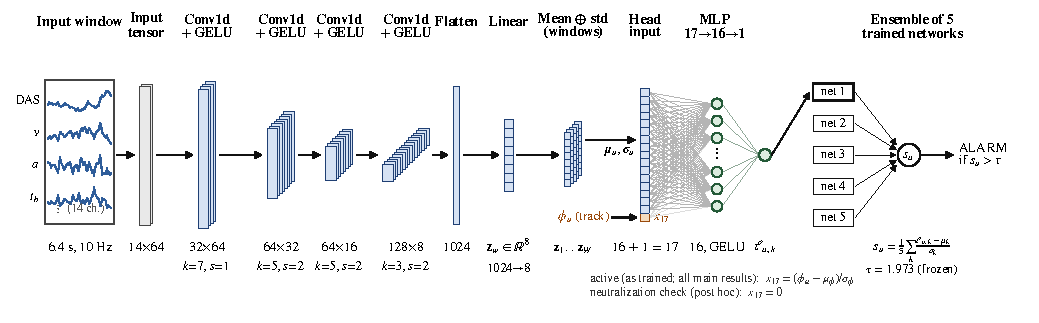
\includegraphics[width=\textwidth]{G0_architecture_two_options}
\caption{\EDIV{} at inference. A 6.4\,s window of the fused track ($14\times64$; left: a real normal window, 4 channels shown) passes four Conv1d+GELU layers (rectangle height $\propto$ time bins, number of rectangles $\propto$ channels; $k$ kernel, $s$ stride), a flatten and a linear projection to $\mathbf z_w\in\mathbb R^8$. The codes of all windows of a track are pooled into mean and standard deviation (16 learned features) for the trained 17--16--1 head; five independently trained networks are standardised with frozen $\mu_k,\sigma_k$ and averaged. The 17th head input $x_{17}$ (amber) is the standardised $\phi_u$ in the model as trained and tested (all main results) and 0 in the post-hoc neutralization check. No truth channel is an input to the networks (\S\ref{sec:disc}).}\label{fig:pipe}\end{figure*}
\section{Data}
\textbf{Sources.} Everything comes from SimStudio, used unchanged. The simulator steps at 50\,Hz; the DAS model emits detections at 30\,Hz, cameras at 10\,Hz with drops, GPS at 1\,Hz. A Kalman filter per track fuses them and exports 50\,Hz state rows. No simulator-truth channel enters the network: truth is dropped at import and used only to \emph{label} vehicles and to verify that an injected anomaly actually happened. The exported tracks themselves, however, are produced by the simulator's tracker, whose association and initialisation may draw on truth; this affects all detectors equally and is discussed in \S\ref{sec:disc}.
\textbf{Network input.} Rows are averaged into 0.1\,s bins (10\,Hz) and map-matched to the lane: eight kinematic channels (longitudinal speed and acceleration, lateral offset and velocity, speed-limit ratio, gap, time headway and closing speed to the vehicle ahead), five sensor-presence masks and the DAS log-amplitude, 14 channels in all. A track is usable with $\ge32$ valid bins and a label-free quality gate; a decision needs $\ge3$ windows.
\textbf{Normal driving.} 1{,}775 exports (148 map regions $\times$ 12 traffic/coverage scenario types, one missing), 14{,}423 tracks. Regions are split spatially with a one-tile buffer: 98 train, 21 val\_A (model selection), 21 val\_B (thresholds only), 8 test.
\textbf{Anomalies.} Nine types: speeding, reckless, hard braking, stalled, weaving, straddling, tailgating, collision, overweight. An injected vehicle is labelled only if a truth rule confirms the effect (a stop of $\ge10$\,s is a stall; a \emph{legitimate} stop lasts $\ge1$\,s and $<10$\,s with deceleration $<4$\,m/s$^2$ and is labelled normal; tailgating is headway $<0.8$\,s for $\ge5$\,s). Unrealised runs are excluded, never relabelled. The sets built during the project (cross-region anomalies, two tailgating sets, a stall set with three stop modes, a legitimate-stop set, a targeted-data set) are listed with their roles in the release. Three result classes are kept apart throughout: \dev{} (nine diagnostic cases, one per type, used for design), \val{} (val\_A sets, used to select models) and the \ft{} (8 test regions, plan frozen before simulation, run once).


\section{The model}
Figure~\ref{fig:pipe} shows \EDIV. The encoder is the 1-D convolutional encoder of the proposal's autoencoder, pre-trained to reconstruct normal windows and then fine-tuned with the head. A usable track is cut into windows of $T=64$ bins (6.4\,s) with stride 8; the encoder maps each window to an 8-d code. For a unit $u$ (one track in deployment; all tracks of one simulated vehicle in the \dev{}/\val{} tables) the codes are pooled into their mean and standard deviation, standardised with constants fitted on training normals, concatenated with one explicit physical summary, the tailgating fraction $\phi_u$ (share of valid bins with a leader, headway $<0.8$\,s and speed $>5$\,m/s, computed from the tracks, not from truth), and passed to a small MLP head that outputs a logit $\ell_u$. Headway and the leader mask are also encoder inputs, so $\phi_u$ summarises over the whole track what the encoder sees window by window; the model is a hybrid of a learned encoder and this one summary. A fixed preprocessing step removes a tracker artefact (a ``leader'' closer than 1\,m at $>5$\,m/s is a duplicate track). Five seeds $k$ are trained with the same recipe; each logit is standardised by the mean and standard deviation of that seed's logits on the 1{,}242 val\_B normals, and the ensemble score is their mean:
\begin{equation}
 z_{u,k}=\frac{\ell_{u,k}-\mu_k}{\sigma_k},\quad s_u=\frac{1}{5}\sum_{k=1}^{5} z_{u,k},\quad \text{ALARM}\iff s_u>\tau,
\end{equation}
with $\tau=1.9726$ the 99th percentile of $s_u$ on the same val\_B normals, i.e.\ a nominal 1\,\% false-alarm rate. Thresholds come only from val\_B and are never copied between models. Table~\ref{tab:hp} gives the frozen recipe; each seed has 67{,}225 trained parameters. \textbf{Two inference options.} \emph{Active} is the hybrid as trained, selected and tested; all main results are for it. \emph{Neutralized} holds the standardised $\phi_u$ input at 0 on the same frozen weights, $\mu_k$, $\sigma_k$ and $\tau$. It measures dependence on $\phi_u$, is not a network trained without $\phi_u$, and was defined after the final test had been exposed (\S\ref{sec:disc}). Two frozen baselines are compared on identical data: the \emph{supervised single model} (one seed, no artefact cleaning, no $\phi$; its own val\_B P99) and the \emph{SimStudio Z-score} as shipped (156 features, 13 of which use truth position error; a truth-free variant gives the same macro recall).

\begin{table*}[t]\centering\footnotesize\setlength{\tabcolsep}{3pt}
\caption{Hyper-parameters of the final model (per seed) and of the autoencoder pre-training that initialises its encoder.}\label{tab:hp}
\begin{tabular}{@{}llll@{}}\toprule
Input & 14 channels $\times$ 64 bins (6.4\,s), stride 8 bins & Batch & 48 normal + 16 anomalous vehicles, $\le$32 windows each \\
Encoder & Conv 14--32--64--64--128 (k 7,5,5,3), Linear 1024$\to$8 & Optimiser & AdamW, lr $10^{-4}$ encoder / $10^{-3}$ head, wd $10^{-4}$ \\
Pooling, head & mean$\oplus$std of codes (16) $\oplus\ \phi$; MLP 17--16--1, GELU & Schedule & 120 steps $\times$ $\le$25 epochs, patience 6, grad.\ clip 5 \\
Loss, selection & BCE per vehicle; checkpoint = best validation AP (val\_A) & Training set & 6{,}761 normal / 105 anomalous vehicles ($\ge$3 windows) \\
Ensemble & seeds 0--4; $\mu_k,\sigma_k$ on 1{,}242 val\_B normals; $\tau$ = P99 & Size & 67{,}225 trained parameters per seed \\\midrule
AE pre-training & 14 inputs, 7 masked targets, bounded decoder, masked MSE & AE schedule & AdamW lr $10^{-3}$, batch 256, $\le$100 epochs, pat.\ 10 \\\bottomrule
\end{tabular}\end{table*}

\section{How the method changed, and why}\label{sec:studies}
Every comparison was pre-registered: the data, the single difference between arms and the replacement rule were written before any simulation or training, and frozen artefacts were hash-checked before and after each round. Full records are in the release (\texttt{research/01}--\texttt{08}). Figure~\ref{fig:ctrl} shows the three comparisons that change one factor each.

\begin{figure*}[t]\centering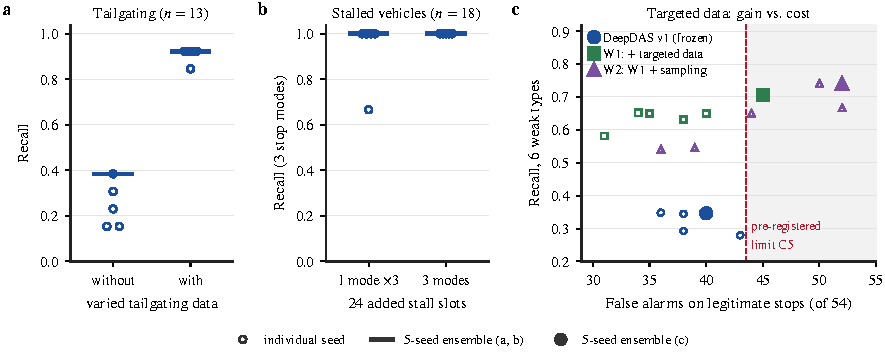
\includegraphics[width=\textwidth]{V5_controlled_comparisons_3panel}
\caption{Controlled comparisons, \val{} only; each panel changes one factor and shows every seed. (a) The same recipe (with $\phi_u$) without and with the varied tailgating data. (b) Both arms add the same 24 stall slots, one stop mode three times or three modes; both ensembles reach 18/18, but one repeated-mode seed falls to 0.67. (c) Weak-type recall against false alarms on 54 legitimate stops for the frozen model and the two targeted-data arms; both cross the pre-registered limit C5.}\label{fig:ctrl}\end{figure*}

\subsection{Reconstruction error does not separate the anomalies}
\emph{Hypothesis (the proposal).} A narrow-bottleneck ConvAE trained on normal windows separates anomalies by reconstruction error. \emph{Test.} The proposed design (13 channels, $T=64$, $d=8$, P95 window error per track, P99 threshold on val\_B) against the Z-score on the 9 published scenarios and an 81-run severity study (9 types $\times$ 3 levels $\times$ 3 seeds) in the test regions. \emph{Result.} AUROC 0.598 [0.52, 0.67] vs 0.887 [0.84, 0.93]; 1 of 91 injected vehicles at a 1\,\% false-alarm rate vs 44\,\%; only speeding at twice the limit crosses the normal P99. The sensitivity analyses the proposal promised were run at this stage: seeds ($\pm0.01$), window length 3.2--12.8\,s and bottleneck 4--32 all leave AUROC at 0.58--0.61; a wider code reconstructs normal \emph{and} anomalous windows better, so the threshold and the anomaly scores fall together. (A DAS-noise sweep was not possible without changing the simulator; stratifying tracks by their DAS noise level showed no dependence.) \emph{Why.} The simulator's anomalies lie inside the normal envelope of a 6.4\,s window: stops, braking up to 4\,m/s$^2$, drift up to 1.8\,m and 1.2\,s headways are all normal driving, and the error criterion discards what the window mean does not carry. \emph{Decision.} Keep the encoder, drop the criterion. These stage-1 numbers are taken from the archived study report; the release ships the checkpoint but does not regenerate them.

\subsection{From latent representation to supervision}
A latent score (max $|z|$ of the pooled code statistics against training normals) already detected 5 of the 9 \dev{} cases without any label, which showed that the encoder organises the codes informatively. The proposal's premise that supervision is impractical holds for field data, but the simulator labels by construction, so a supervised test became possible. A head on the encoder, trained on 34 anomalies simulated in regions disjoint from the evaluation regions (\emph{cross-region}; earlier anomaly scenes had shared regions with the test normals), detected 7 of 9. Supervision does not remove the labelling constraint of real deployments; it removes it inside the simulator.

\subsection{Seed sensitivity leads to an ensemble}
The same recipe with seeds 0--2 detected 7, 2 and 3 of the 9 \dev{} cases: with 105 positives, head initialisation and batch order matter as much as the data. Five standardised seeds (Eq.~1) are averaged from here on; every later comparison is ensemble-level, with per-seed spread reported.

\subsection{Diversity of data, not repetition}
Diagnosing the single model's misses had shown that headway is in its input but not exposed by mean/std pooling, so $\phi_u$ was proposed as an explicit summary (study 02). With the early data it was not enough: the development tailgating case stayed undetected with and without $\phi_u$ (0/3 seeds each). \emph{Hypothesis:} too few \emph{realised}, varied examples. Four versioned plans produced 59 verified tailgaters (shared planned routes, varied leader speed and episode length, and matched controls that drive the same route at the default headway). With them the ensemble's \val{} tailgating recall rose from 0.385 to 0.923 (Fig.~\ref{fig:ctrl}a); both arms included $\phi_u$, and the expanded data without $\phi_u$ was not trained. The new data cost the stalled case: tailgating took $\approx$60\,\% of positive draws and all training stalls were one mode (move--stop 30\,s--move). Balancing types or freezing the encoder did not help. \emph{Hypothesis:} missing stop \emph{modes}. Two arms added 24 stall slots each, the same mode three times or three modes (standing from $t=0$, stop until the end, move--stop--move), with identical controls and legitimate stops. Diversity reached 18/18 on stall validation for every seed (repetition: 0.93 $\pm$ 0.15 per seed) and won the tie-break on validation AP (0.781 vs 0.751; Fig.~\ref{fig:ctrl}b). This ensemble is \EDIV.

\subsection{Targeted data doubles weak-type recall but is not adopted}\label{sec:w12}
The selected model flagged 40 of 54 legitimate ($<10$\,s) stops in validation. A read-only diagnosis isolated the cause (\S\ref{sec:disc}); two pre-registered remedies (controlled exposure; a temporal branch over the window sequence) and an epoch-selection rule each reduced the alarms but broke another condition, so the model was left unchanged. After the final test, a diagnosis on its (now exposed) runs showed that for the six weak types the information is present in the input and in the encoder (linear-probe AUC 0.81--1.0) but lost in the head, which had seen four homogeneous examples per type. We pre-registered one last round: 314 new runs with wide parameter grids per weak type and matched legal controls, two arms (W1: data only; W2: exposure-preserving sampling), and nine conditions including C5, at most three more legitimate-stop alarms than the reference. Both arms doubled weak-type recall and failed only C5 (Fig.~\ref{fig:ctrl}c); neither was promoted, and because the final test had informed their design, no final-test number exists for them.

\begin{figure*}[t]\centering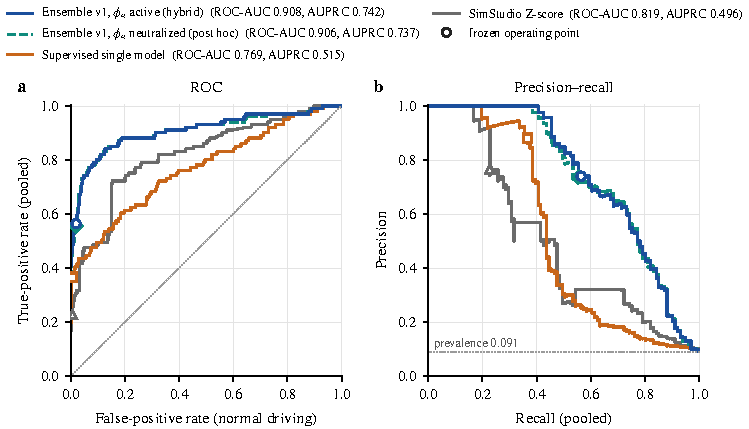
\includegraphics[width=0.8\textwidth]{G4_roc_pr_four_configurations}
\caption{Final test, common decided subset (101 anomalies, 1{,}008 normal vehicles): (a) ROC, (b) precision--recall; open markers: frozen operating points. The hybrid (\EDIV, $\phi_u$ active), the single model and the Z-score were frozen before the test; the $\phi_u$-neutralized curve (dashed) is a post-hoc analysis of the exposed test.}\label{fig:roc}\end{figure*}
\begin{figure}[t]\centering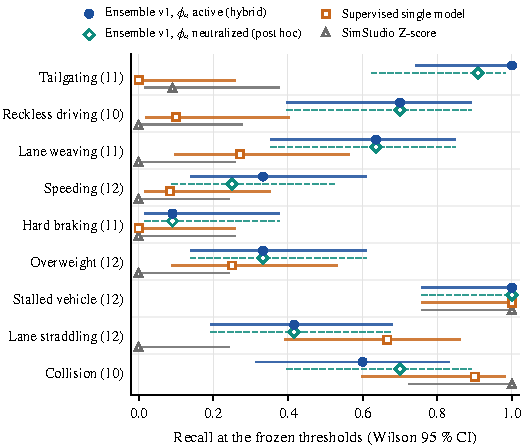
\includegraphics[width=\columnwidth]{G3_detection_by_type_four_configurations}
\caption{Final-test recall per anomaly type at the frozen thresholds (common decided subset, $n$ in brackets, Wilson 95\,\% intervals). The $\phi_u$-neutralized option is post hoc. The deep models detect behaviours the Z-score was blind to; hard braking is weak for all detectors (at most 1/11).}\label{fig:type}\end{figure}
\section{Results}
\textbf{Development (not independent).} \EDIV{} detects 8 of the 9 \dev{} cases (overweight scores 1.865 against $\tau=1.973$); the single model 7, missing weaving and tailgating.
\textbf{Validation (used for selection).} Macro recall over the nine types 0.714, AP 0.781, stall validation 18/18, tailgating 12/13, false alarms on val\_A normal driving 1.07\,\%, legitimate stops 40/54; per-seed macro recall 0.55--0.76.
\textbf{Final test.} 228 runs in the 8 test regions with new scenes, background traffic, seeds and injection lanes; plan, models, thresholds and evaluation code frozen before simulation and run once; 105 of 108 core injections realised. The test is independent for the three detectors frozen before it (\EDIV, the single model, the Z-score); after its results were exposed it was also used for the diagnosis that motivated W1/W2 (\S\ref{sec:w12}), so it is not an independent test for any model trained afterwards. Decisions are per usable track; a vehicle counts as detected if any decided track alarms. Table~\ref{tab:ft} compares the detectors on the vehicles decided by all of them, because coverage differs: the deep models decide 1{,}008 of 1{,}708 normal vehicles (134 untracked, 320 without a usable track, 246 with $<3$ windows), the Z-score 1{,}574. \EDIV{} reaches macro recall 0.568 against 0.364 and 0.232; paired exact McNemar tests on the pooled anomalies give 38 vs 4 discordant detections against the Z-score ($p<0.001$) and 28 vs 8 against the single model ($p=0.0012$). In Fig.~\ref{fig:roc} the hybrid ensemble lies above both baselines across thresholds. Figure~\ref{fig:type} shows where the gain is: tailgating 11/11 and weaving 7/11 (Z-score 1/11 and 0/11), reckless 7/10; stalls 12/12 for all three. Hard braking (1/11), speeding (4/12) and overweight (4/12) remain weak, and on straddling (5/12) and collision (6/10) the single model is better. False alarms on normal driving are 2.0\,\% (1.3\,\% without the tailgating controls), 0.5\,\% and 0.7\,\%; on legitimate stops 20/28 (3\,s 3/8, 5\,s 8/11, 8\,s 9/9), 14/28 and 22/28; on tailgating matched controls 7/11, 0/11, 0/12, although within each pair the tailgater always scores higher.
\textbf{W1/W2 (validation only).} On the expanded validation set weak-type recall rose from 0.35 to 0.71 (W1) and 0.74 (W2) and ROC-AUC from 0.87 to 0.96, with normal-driving false alarms unchanged ($\approx$1\,\%) and tailgating-control alarms reduced (6/7 $\to$ 0/7, 2/7); legitimate-stop alarms rose to 45 and 52 of 54 against a limit of 43. These sets hold 9--10 vehicles per weak type, so one detection moves recall by 0.1, but the ranking is stable across seeds (every W1 seed gains $\ge0.28$).

\begin{table}[t]\centering\footnotesize\setlength{\tabcolsep}{1.6pt}
\caption{Final test (independent for the three frozen detectors), common decided subset (101 anomalies, 1{,}008 normal vehicles). Macro recall with 95\,\% bootstrap CI over runs. On its own larger decided set (105 anomalies, 1{,}574 normals) the Z-score has ROC-AUC 0.783, AUPRC 0.394, precision 0.64, F1 0.33.}\label{tab:ft}
\begin{tabular}{@{}lccc@{}}\toprule
 & Ens.\ v1 (hybrid) & Single & Z-score \\\midrule
Macro recall & \textbf{0.568} [.49,.65] & 0.364 [.30,.43] & 0.232 [.22,.26] \\
Precision / F1 & 0.74 / \textbf{0.64} & 0.88 / 0.52 & 0.77 / 0.35 \\
ROC-AUC / AUPRC & \textbf{0.908} / \textbf{0.742} & 0.769 / 0.515 & 0.819 / 0.496 \\
FA, normal driving & 20 (2.0\,\%) & 5 (0.5\,\%) & 7 (0.7\,\%) \\
FA, legit.\ stops (of 28) & 20 & 14 & 22 \\
Decided normals of 1{,}708 & 1{,}008 & 1{,}008 & 1{,}574 \\\bottomrule
\end{tabular}\end{table}


\section{Discussion}\label{sec:disc}
\textbf{What the detour taught us.} Reconstruction error measures what a bounded, narrow model cannot reproduce; here the anomalies are reproducible within a window, so the score tracks severity only for the 2$\times$ speeders. The encoder nevertheless learned a useful representation, and the decisive methodological step was not a new architecture but \emph{verified} labels from the simulator, strict separation of evaluation regions and scenes, and pre-registered decisions. Twice the same lesson on data: tailgating needed realised, varied episodes with matched controls, and stalls needed three stop modes; tripling one mode gave 0.93 $\pm$ 0.15 per seed where diversity gave 1.00 $\pm$ 0.00.
\textbf{Legitimate versus abnormal stops.} Removing the windows that overlap the truth stop removes every alarm, so the stop itself drives the score; mean/std pooling makes the \emph{share} of stop windows decide; the tracker compresses stop duration (a 30\,s truth stop shows $\approx$9\,s); and the 23 training legitimate stops supplied about 105$\times$ fewer stop windows than the stalls. Three remedies reduced the alarms (37, 27 and 21 of 54), none within the other constraints, and the final test confirmed the problem (8\,s stops 9/9). This is the model's main limitation and was not resolved.
\textbf{Contribution of the headway summary.} We compared the frozen hybrid with the same model when $\phi_u$ is neutralized at inference (Table~\ref{tab:phi}). The comparison measures dependence on the feature, not the performance of a network trained without it, and the final-test rows are post hoc. With $\phi_u$ active the frozen model detects one more development case, the tailgating case (score 3.73 vs $-0.08$; its $\phi_u=0.81$ lies 25 standard deviations above the training-normal mean). Most final-test tailgaters stay detected when it is neutralized, and a linear probe on the 16 pooled code statistics separates them from normal tracks (AUC 1.0, study 06), so the learned representation carries most of their signal. Other development scores move by $\le$0.03; normal-driving false alarms are unchanged (20/1{,}008); speeding and collision change by one vehicle each. This does not show that the tailgating gain came from $\phi_u$ alone or from the data alone: the expanded data without $\phi_u$ was never trained.
\begin{table}[h]\centering\footnotesize\setlength{\tabcolsep}{3pt}
\caption{Dependence of the frozen ensemble on $\phi_u$ (inference-time intervention; same weights and frozen $\tau$).}\label{tab:phi}
\begin{tabular}{@{}lcc@{}}\toprule
Check & $\phi_u$ neutralized & $\phi_u$ active \\\midrule
Nine development cases & 7/9 & 8/9 \\
Tailgating, validation & 9/13 & 12/13 \\
Tailgating, exposed test (post hoc) & 10/11 & 11/11 \\
Macro recall, exposed test (post hoc) & 0.560 & 0.568 \\\bottomrule
\end{tabular}\end{table}
\textbf{Why hard braking and mild speeding stay weak.} The tracker's longitudinal acceleration has a median minimum of $-7.5$\,m/s$^2$ on \emph{normal} tracks, above the injected 6\,m/s$^2$ brake, so the brake is inside the noise; and the simulator's normal traffic reaches 1.10--1.12$\times$ the limit, so mild speeding overlaps normal driving by construction. These are measured properties of the data, not hypotheses. Encoder probes of 0.91--1.0 against head AUCs of 0.80--0.93 locate the remaining loss after the encoder, where four examples per type were the cause we could act on; W1/W2 confirmed it at a price.
\textbf{Coverage and realism.} The deep models give no decision for 700 of 1{,}708 normal vehicles (41\,\%), set by the tracker and the $\ge3$-window rule; undecided vehicles never count as normal. Although no truth channel is an input to the deep networks (unlike the Z-score's 13 truth-error features), the exported tracks inherit truth through the tracker's association and initialisation, so all detectors see cleaner tracks than a real system would. The one real DAS recording (Klausner street: a bus standing $\approx$31\,s, a stall by our $\ge10$\,s rule) is detected by \EDIV{} in both options ($s_u=4.53$ / $4.55>\tau$) and by the Z-score; the stage-1 autoencoder missed it. One case is not a recall estimate.

\section{Limitations and future work}
(1) False alarms on legitimate short stops and on tailgating matched controls. (2) Weak recall on hard braking, speeding, overweight and straddling; W1/W2 show it is learnable but not within the stop constraint. (3) Decision coverage set by the tracker. (4) The final test is independent only for the models frozen before it; its exposed results informed the W1/W2 diagnosis and design, so W1/W2 have no independent number and a later model needs a new test. (5) Simulation only, except one real track (detected). (6) The severity and sensitivity analyses exist for the autoencoder stage only. (7) The separate contributions of $\phi_u$ and of the tailgating data are not identified; that needs a 16-input head retrained on the final data. Future work: a duration-aware stop feature or post-filter computed from the track, a tracker that preserves stop duration, and a labelled real recording; the release provides the frozen baseline such work must beat.

\section{Reproducibility}
The self-contained release \texttt{DeepDAS\_Release\_v1.0} (PyTorch 2.14, CPU) holds the processed data, the frozen checkpoints and thresholds, the code, the seven study records and a verification script: \texttt{pip install -r requirements.txt}, then \texttt{python scripts/verify\_release.py} regenerates the development table, all validation scores and the final-test tables and compares them with the shipped results (byte-identical on x86-64; identical decisions and tables on aarch64). Stage-1 and study numbers (\S\ref{sec:studies}) come from archived records. Retraining the five seeds reproduces the checkpoints bit-exactly on the build platform. Raw simulations (4.5\,GB) are a separate hashed package. The review copy \texttt{DeepDAS\_Release\_v1.1\_review} adds \texttt{-{}-phi-mode active|neutralized} and \texttt{research/08}.

\balance
\section*{Team contributions}
\textcolor{note}{[To be completed by the authors: contribution of Noa Sapir; contribution of Asaf Zini; contribution of Neta Shaboo.]}

\section*{Code}
\url{https://github.com/noasapir3/Deep-DAS} (data: release \texttt{data-v1.0}).

\footnotesize
\begin{thebibliography}{9}\setlength{\itemsep}{0pt}
\bibitem{lindsey2021} N.~J. Lindsey and E.~R. Martin, ``Fiber-optic seismology,'' \emph{Annu. Rev. Earth Planet. Sci.}, vol.~49, pp. 309--336, 2021.
\bibitem{ye2023} Z.~Ye \emph{et al.}, ``Traffic flow and vehicle speed monitoring with the object detection method from the roadside distributed acoustic sensing array,'' \emph{Front. Earth Sci.}, vol.~10, 992571, 2023.
\bibitem{robles2025} I.~Robles-Urquijo \emph{et al.}, ``Method to use transport microsimulation models to create synthetic distributed acoustic sensing datasets,'' \emph{Appl. Sci.}, vol.~15, no.~9, 5203, 2025.
\bibitem{sakurada2014} M.~Sakurada and T.~Yairi, ``Anomaly detection using autoencoders with nonlinear dimensionality reduction,'' in \emph{Proc. MLSDA Workshop}, 2014.
\bibitem{audibert2020} J.~Audibert \emph{et al.}, ``USAD: Unsupervised anomaly detection on multivariate time series,'' in \emph{Proc. ACM KDD}, 2020.
\bibitem{ruff2021} L.~Ruff \emph{et al.}, ``A unifying review of deep and shallow anomaly detection,'' \emph{Proc. IEEE}, vol.~109, no.~5, pp. 756--795, 2021.
\bibitem{pang2021} G.~Pang, C.~Shen, L.~Cao, and A.~van den Hengel, ``Deep learning for anomaly detection: A review,'' \emph{ACM Comput. Surv.}, vol.~54, no.~2, 2021.
\bibitem{lakshminarayanan2017} B.~Lakshminarayanan, A.~Pritzel, and C.~Blundell, ``Simple and scalable predictive uncertainty estimation using deep ensembles,'' in \emph{Proc. NeurIPS}, 2017.
\bibitem{wu2023} R.~Wu and E.~Keogh, ``Current time series anomaly detection benchmarks are flawed and are creating the illusion of progress,'' \emph{IEEE Trans. Knowl. Data Eng.}, vol.~35, no.~3, pp. 2421--2429, 2023.
\bibitem{kaufman2012} S.~Kaufman, S.~Rosset, C.~Perlich, and O.~Stitelman, ``Leakage in data mining: Formulation, detection, and avoidance,'' \emph{ACM Trans. Knowl. Discov. Data}, vol.~6, no.~4, 2012.
\end{thebibliography}
\end{document}
